% Unified chapter derived from the Team 4 source and maintained in this project.
\chapter{Production and Cost Forecasting}
\chapterstatus{Team 4 operating methodology refreshed with Barrick Q1--Q2 2026 actuals; price simulation and valuation demonstrator excluded.}
\sourceassetnote
\section{Introduction, Data and Definitions}
\subsection{Overview}
The accurate valuation of mining assets fundamentally relies on the precise estimation of future Cost of Sales (CoS). However, projecting these operational costs over a medium term horizon, specifically five years (or 20 quarters), presents significant statistical hurdles, most notably the management of variance within highly volatile commodities markets. When applied to isolated mining operations, standard econometric models frequently generate confidence intervals that are prohibitively wide for practical financial modeling, occasionally yielding illogical outputs such as negative costs or exponential growth trajectories. To mitigate these structural limitations, this paper introduces a hybrid Log-Space SARIMA framework.

Complementary to the cost side, the second pillar of operational profitability is gold production, the primary driver of the firm's revenue stream. Forecasting total output as a single time series is unsatisfactory: the heterogeneity of individual assets and the compounding of mine-specific shocks degrade the signal-to-noise ratio and inflate the resulting confidence intervals. To address this, we adopt a bottom-up physical decomposition into Ore Processed, Average Grade, and Recovery Rate, with the first two forecast through mine-level SARIMA models and the third simulated within historically observed operational bounds. Aggregate uncertainty is then evaluated using Goodman's exact variance-of-products approximation, which preserves the multiplicative structure of the production formula while avoiding the explosive variance of a naive product of confidence intervals.

Gold price risk is deliberately outside this chapter. The operating forecasts produced here are handed to the independent Team~8 price layer and to the unified DCF only after production and Cost of Sales have been constructed. This separation prevents the historical Team~4 price demonstrator from being confused with the gold scenarios and corporate valuation used in the unified experiment.
\subsubsection{Objective}
The objective is to build a five-year operating contract for Barrick's production and Cost of Sales. Due to the compounding volatility inherent in the mining sector, traditional top-down forecasting models frequently generate explosive variances and operationally impossible scenarios, such as negative costs or unbounded production. To resolve these structural limitations, this chapter proposes a bottom-up model. By decomposing operating performance into geological and metallurgical drivers, the approach aims to stabilise medium-term cost and production forecasts without producing a standalone price or valuation result.
\subsubsection{Data Sources}
All the non-market data used in this analysis were extracted from Barrick Gold Corporation's quarterly reports, available as PDF and/or Excel files on the company's investor website. The dataset concentrates on Barrick's largest gold mines; copper operations and smaller mines were excluded because they have a negligible impact on total production and revenue for the periods considered.

The mines included in the analysis are:
\begin{itemize}
  \item Bulyanhulu, Carlin, Cortez, Kibali, Loulo--Gounkoto, North Mara, Pueblo Viejo, Turquoise Ridge.
\end{itemize}
\subsubsection{Definitions of Financial and Process Metrics}
To ensure clarity in valuation, we adopt the standard definitions provided in the Barrick Annual Report 2024 \sourcecitation{barrick2024}.

\begin{definition}[Cost of Sales (Gold)]
Cost of sales applicable to gold production includes site operating costs, royalty expense, depreciation, and community relations costs. It excludes costs associated with sites in closure or care and maintenance. On a per-ounce basis, it is calculated as the cost of sales across operations divided by ounces sold (attributable basis).
\end{definition}


\begin{definition}[Ore tonnes processed]
Total physical volume of ore (gold-bearing rock) measured in tonnes, that has been extracted from the mine and fed into the processing plant.
\end{definition}

\begin{definition}[Average grade]
Concentration or richness of gold (measured in grams/tonne) within the ore that's being processed.
\end{definition}

\begin{definition}[Recovery rate]
Percentage of gold present in the ore successfully extracted. It measures the efficiency of the processing facilities.
\end{definition}

% ===============================
% Chapter : Methodology
% ===============================
\section{Cost of sales forecast methodology}
This chapter details the forecasting algorithm implemented in R. Before defining the final "Log-Space Delta-Anchor" model, we outline the investigative process and alternative approaches that were discarded, justifying the necessity of the chosen methodology. The data utilized for this study was gathered from Barrick Gold's quarterly reports for the selected mines previously mentioned in the introduction. Although historical data for certain mines extends back to 2016, a complete, continuous dataset devoid of missing values (NaNs) across all selected mines is only available from 2019 onward. Consequently, to ensure data integrity and consistency, only data from 2019 onwards has been used for the following analysis \sourcecitation{githubrepo}.

% Asset/code block omitted pending provenance acceptance.
\subsection{Evolution of the Modeling Strategy}
The development of the valuation model proceeded through three distinct iterations. The challenges encountered in the first two approaches directly informed the design of the final Global Master Chain framework.

\paragraph{Attempt 1 -- Fundamental Factor Modeling:}
Our initial approach aimed to construct a formal explanatory model based on the primary cost drivers identified in Barrick Gold's annual reports. Management explicitly lists \textbf{diesel prices, labor costs, and currency exchange rates} as the most significant factors impacting the Cost of Sales.

We attempted to model the Cost of Sales ($Y_t$) as a function of these exogenous variables:
\[ Y_t = \beta_0 + \beta_1(\text{Oil}_t) + \beta_2(\text{Labor}_t) + \beta_3(\text{FX}_t) + \varepsilon_t \]

However, this approach proved unfeasible for two reasons:
\begin{enumerate}
    \item \textbf{Data Granularity and Geography:} The mines are geographically dispersed across vastly different jurisdictions (e.g., Nevada, USA vs. Loulo--Gounkoto, Mali). Obtaining reliable, high-frequency historical data for local labor costs or specific energy tariffs in developing regions was extremely difficult.
    \item \textbf{Propagation of Uncertainty:} To forecast mining costs 5 years into the future, we would first need to forecast the drivers (e.g., the price of Brent Crude in 2029). The error associated with forecasting these macroeconomic indicators, combined with the model error, led to an explosion of uncertainty in the final output.
\end{enumerate}

\paragraph{Attempt 2 -- Idiosyncratic Univariate Forecasting:}
We subsequently moved to univariate time series models, applying standard forecasting algorithms directly to the data of each individual mine. We tested: ETS (Error, Trend, Seasonality) and Holt-Winters Exponential Smoothing.\\
Those failed due to sample size limitations. The reliable dataset covers the period from Q1 2019 to Q4 2025, providing approximately $N \approx 24$ data points per mine. Given the high operational volatility of individual sites (due to maintenance shutdowns, grade variations, or local disruptions), the signal-to-noise ratio was too low. The models frequently failed to converge or produced confidence intervals so wide that they encompassed negative costs, rendering them useless for valuation.

\paragraph{Final Approach -- The Global Master Chain Hypothesis:}

By overlaying the time series of all major mines (fig \sourceref{fig:ts overlay}) on a single plot, we observed synchronicity in the movements of Cost of Sales, particularly when analyzing relative changes rather than absolute dollar amounts. 

To statistically validate this visual intuition \sourcecitation{hair2018}, we analyzed the quarter-over-quarter cost shocks of the mines. The dataset was strictly filtered to include only data from 2019 onwards, ensuring a complete, balanced panel across all operations and cleanly capturing the recent era of heightened macroeconomic volatility.

First, a \textbf{Bartlett's Test} \sourcecitation{hair2018} was conducted on the correlation matrix of the mines' percentage cost changes. The test yielded a statistically significant result (\textbf{p-value = 0.0186}), allowing us to cleanly reject the null hypothesis that the mines' cost structures evolve independently.

Subsequently, a \textbf{Principal Component Analysis} (PCA) was performed to isolate and quantify this shared momentum \sourcecitation{hair2018}. The results provided robust quantitative support for the Global Master Chain Hypothesis: the first principal component (PC1) alone explains \textbf{41.22\% }of the total variance in cost shocks across the dataset. Furthermore, the first two principal components combined account for nearly 63\% (62.79\%) of all cost fluctuations, confirming a heavily macro-driven environment.

% Asset/code block omitted pending provenance acceptance.


In a real-world operational context, where individual physical assets are subject to severe local disruptions (e.g., distinct labor strikes, regional weather events, and varying ore grades), discovering that over 40\% of all cost volatility is dictated by a single, shared principal component is highly significant \sourcecitation{hair2018}.

This observation provided the empirical justification to adopt a Log-Space Beta scaling Anchor approach. This method consists of aggregating all mines to extract a stable global signal (the "Master Chain"), forecasts this stable signal, and then projects the trend back onto individual mines using a volatility scalar ($\beta$).

\subsection{Rationale for Logarithmic Transformation}
To implement this Global Master Chain, we apply a natural logarithm transformation to the Cost of Sales ($Y_t$). This step is critical for three econometric reasons specific to financial time series.

Financial time series often exhibit heteroscedasticity, where the volatility of the series increases as the level of the series rises. In mining, as input costs (energy, labor, steel) rise, the absolute dollar variance of the Cost of Sales tends to increase.

Standard linear models assume homoscedasticity (constant variance). By modeling $\ln(Y_t)$ rather than $Y_t$, we stabilize the variance, making the series more amenable to ARIMA modeling.

Inflation and cost escalation are inherently multiplicative processes. If costs grow by rate $r$, the process is defined as:
\[ Y_t = Y_{t-1} \cdot (1+r) \]
Linear models (like ARIMA) are additive. The logarithmic transformation converts this multiplicative relationship into a linear additive one:
\[ \ln(Y_t) = \ln(Y_{t-1}) + \ln(1+r) \]
This allows the linear SARIMA model to capture percentage growth rates rather than absolute dollar increments.

A standard Gaussian forecast on raw data ($Y_t$) carries a non-zero probability of predicting negative costs if the variance is sufficiently high or the trend is downward. By forecasting in log-space and exponentiating the result ($\hat{Y} = e^{\ln \hat{Y}}$), we mathematically guarantee that the forecasted Cost of Sales will strictly be non-negative ($\hat{Y} > 0$).
\subsubsection{The Global Master Chain (Log-Space)}
\begin{definition}[Log-Global Master Chain - Weighted]
Let $Y_{i,t}$ be the Cost of Sales for mine $i$ at time $t$. Let $Q_{i,t}$ represent the quantity extracted (e.g. ounces produced) for mine $i$ at time $t$. We first compute the weighted cross-sectional average $\bar{Y}_t$ by weighting each mine's cost by its relative production volume, and then apply the natural logarithm to obtain the master chain $M_t$:
\[
M_t = \ln(\bar{Y}_t) = \ln\left( \frac{\sum_{i=1}^{N} Q_{i,t} Y_{i,t}}{\sum_{i=1}^{N} Q_{i,t}} \right)
\]
\end{definition}
\subsection{SARIMA Model, Results and Validation}
Having established the Global Master Chain as a reliable proxy for the shared cost momentum across all mining operations, the next critical step is to forecast its future trajectory. To accomplish this, we utilize a Seasonal Autoregressive Integrated Moving Average (SARIMA) framework \sourcecitation{box1970} as our primary forecasting engine. 

This section details the complete modeling workflow applied to the log-transformed Master Chain. We begin by defining the mathematical structure and the strictly required statistical assumptions of the SARIMA algorithm. Following this theoretical foundation, we present the empirical results: the pre-modeling stationarity tests used to determine the necessary order of integration, the optimal parameter estimation selected via information criteria, and the rigorous residual diagnostics performed to ensure the model's structural validity. Finally, we provide an out-of-sample validation to empirically demonstrate the model's predictive accuracy before deploying it for the final five-year valuation projections.
\subsubsection{Mathematical Formulation of the SARIMA Model}
To forecast the Master Chain $M_t$, we employ a Seasonal Autoregressive Integrated Moving Average (SARIMA) framework. This class of models extends the standard ARIMA structure to explicitly capture both non-seasonal momentum and repeating seasonal cycles inherent in financial and operational time series.


A general $SARIMA(p,d,q)(P,D,Q)_s$ model is defined mathematically as.

\begin{definition}[SARIMA Formulation]
Let $y_t$ represent the observed value of the time series at time $t$. The generalized multiplicative SARIMA model is expressed as:
$$\phi(B)\Phi(B^s)(1-B)^d(1-B^s)^D y_t = c + \theta(B)\Theta(B^s)\varepsilon_t$$

Where the constituent variables and polynomials are defined as follows:
\begin{itemize}
\renewcommand{\labelitemi}{$-$}
    \item $y_t$: The modeled time series (in this context, the log-transformed Master Chain $M_t$).
    \item $B$: The backshift (lag) operator $B^k y_t = y_{t-k}$.
    \item $s$: The seasonal periodicity of the data (e.g., $s=4$ for quarterly financial reporting).
    \item $p, d, q$: The non-seasonal autoregressive order, degree of differencing, and moving average order, respectively.
    \item $P, D, Q$: The seasonal autoregressive order, degree of seasonal differencing, and seasonal moving average order, respectively.
    \item $\phi(B) = 1 - \phi_1 B - \phi_2 B^2 - \dots - \phi_p B^p$: The non-seasonal autoregressive polynomial, capturing the dependency of the current value on its immediate $p$ past values.
    \item $\Phi(B^s) = 1 - \Phi_1 B^s - \Phi_2 B^{2s} - \dots - \Phi_P B^{Ps}$: The seasonal autoregressive polynomial, capturing the dependency of the current value on its past values from $P$ previous seasonal cycles.
    \item $(1-B)^d$: The non-seasonal differencing operator, applied $d$ times to eliminate structural trends and achieve mean stationarity.
    \item $(1-B^s)^D$: The seasonal differencing operator, applied $D$ times to eliminate seasonal drift.
    \item $c$: The constant term or "drift", representing the underlying deterministic growth rate of the differenced series.
    \item $\theta(B) = 1 + \theta_1 B + \theta_2 B^2 + \dots + \theta_q B^q$: The non-seasonal moving average polynomial, modeling the influence of $q$ past forecast errors.
    \item $\Theta(B^s) = 1 + \Theta_1 B^s + \Theta_2 B^{2s} + \dots + \Theta_Q B^{Qs}$: The seasonal moving average polynomial, modeling the influence of past forecast errors from $Q$ previous seasonal cycles.
    \item $\varepsilon_t$: The white noise error term at time $t$, assuming independent and identically distributed innovations where $\varepsilon_t \sim WN(0, \sigma^2)$.
\end{itemize}
\end{definition}

This generalized framework allows the forecasting algorithm to systematically test and isolate both immediate, quarter-over-quarter cost momentum and delayed, year-over-year seasonal dependencies prior to model selection.
\subsubsection{Underlying Statistical Assumptions}
To ensure the mathematical validity of the SARIMA framework and the reliability of its subsequent forecasts, the model relies on several core statistical assumptions regarding the underlying data-generating process:

\begin{itemize}
    \item \textbf{Stationarity:} The time series, post-differencing ($d$ and $D$), must exhibit weak stationarity. This implies that its statistical properties specifically the mean, variance, and autocovariance are constant over time and independent of the specific time $t$ at which they are observed.
    \item \textbf{Linearity:} The model assumes that the current value of the series is a linear combination of its past values (autoregressive terms) and past error shocks (moving average terms).
    \item \textbf{Invertibility and Stability:} The roots of both the autoregressive polynomial $\phi(B)$ and the moving average polynomial $\theta(B)$ must lie strictly outside the unit circle. This guarantees that the model is mathematically stable (i.e., past shocks decay over time rather than explode) and uniquely identifiable.
    \item \textbf{White Noise Innovations:} The error terms (or innovations) $\varepsilon_t$ must be independently and identically distributed (i.i.d.) with a mean of zero and a constant variance $\sigma^2$ (homoscedasticity). Crucially, there must be no serial correlation between the residuals at any lag.
    \item \textbf{Normality of Residuals:} While accurate point forecasts can be generated without strict normality, the calculation of precise and symmetric confidence intervals explicitly assumes that the error terms $\varepsilon_t$ follow a Gaussian (normal) distribution.
\end{itemize}
\subsubsection{Model Selection and Validation}
Model selection was performed using an automated grid-search algorithm optimized for Information Criteria, allowing for both seasonal and non-seasonal terms. The algorithm identified an \textbf{ARIMA(3,1,0) with drift} as the optimal fit, minimizing both the Akaike Information Criterion \sourcecitation{akaike1974} (AIC = -94.64) and the Bayesian Information Criterion \sourcecitation{schwarz1978} (BIC = -86.87). Notably, the algorithm found no significant seasonal patterns to justify the inclusion of seasonal parameters.

The chosen model indicates that the series required first-order differencing ($d=1$) to stabilize the mean, followed by three autoregressive terms ($p=3$) to capture the temporal dependencies. 

The formal mathematical representation of the estimated ARIMA(3,1,0) model with drift, using the backshift operator $B$, is expressed as:

$$(1 + 0.9501B + 0.6128B^2 + 0.3003B^3)(1 - B)y_t = 0.0222 + \varepsilon_t$$

Where $y_t$ represents the log-transformed series, $0.0222$ is the estimated drift constant (representing the underlying linear trend of the differenced series), and $\varepsilon_t$ represents the white noise error term.
\subsubsection{Residual Diagnostics}
To ensure the structural validity of the selected model, the residuals were subjected to diagnostic testing. \\
 \textbf{Autocorrelation (Ljung-Box Test):} The Ljung-Box test \sourcecitation{ljung1978} returned a test statistic of $Q^* = 2.42$ with a p-value of \textbf{0.6585}. Failing to reject the null hypothesis confirms that the residuals do not exhibit significant autocorrelation and behave as independent white noise. \\
\textbf{Normality (Shapiro-Wilk Test):} The Shapiro-Wilk test \sourcecitation{shapiro1965} yielded a p-value of \textbf{0.6826}. This confirms that the residual distribution does not significantly deviate from a normal distribution, ensuring the reliability of the generated confidence intervals for future point forecasts.


To assess practical forecasting performance and guard against overfitting, the model was evaluated on a 12-period hold-out test set. The ARIMA(3,1,0) predictions were benchmarked against a Naive (Random Walk) forecasting model. 

The predictive accuracy was measured using Root Mean Squared Error (RMSE) and Mean Absolute Percentage Error (MAPE). 

% Asset/code block omitted pending provenance acceptance.


The ARIMA model demonstrated vastly superior predictive capabilities on unseen data. It achieved an RMSE three times lower than the benchmark model and maintained a remarkably low MAPE of \textbf{0.603\%}. This out-of-sample performance solidly justifies the use of the ARIMA(3,1,0) model for future predictions of this time series.

% Asset/code block omitted pending provenance acceptance.
\subsection{Volatility Scaling (\texorpdfstring{$\beta$}{beta})}
To project the global master trend onto individual mines, we cannot assume a 1:1 relationship. Some mines exhibit significantly higher operational risk than the global average due to specific geological or geopolitical factors. We estimate a specific volatility scalar, $\beta_i$ \sourcecitation{poon2003}.
\subsubsection{Regularization: Blume's Adjustment }
We define the raw volatility scalar $\beta_{raw,i}$ as the ratio of the standard deviation of the mine's historical log-returns to the standard deviation of the global master chain's historical log-returns.

Let $r_{i,t} = \Delta \ln(Y_{i,t})$ be the log-return of mine $i$, and $r_{global,t} = \Delta M_t$ be the global log-return.
\[
\beta_{raw,i} = \frac{\sigma(r_{i,t})}{\sigma(r_{global,t})}
\]

It is crucial to note that this metric differs from a standard financial Beta (CAPM), which is defined as $\rho_{i,m} \cdot \frac{\sigma_i}{\sigma_m}$. We deliberately exclude the correlation coefficient ($\rho_{i,m}$) from our calculation. In cost forecasting, a low correlation between a specific mine and the global index often indicates high \textit{idiosyncratic} risk (e.g., local strikes, wall collapses) rather than stability. A regression-based Beta would dampen the projected volatility for uncorrelated assets, leading to dangerously narrow confidence intervals. By utilizing the simple ratio of standard deviations, we ensure that the forecast envelope fully reflects the mine's total historical instability, regardless of its correlation with the global cycle.


Given the limited sample size ($N \approx 30$ quarters per mine), the raw $\beta_{raw,i}$ estimates are subject to significant sampling noise. Extreme values (e.g., $\beta > 3.0$) are often artifacts of single outlier events rather than persistent structural characteristics.

To mitigate this, we apply Blume's Adjustment \sourcecitation{blume1975}, a shrinkage technique used in finance to adjust beta estimates towards the market mean of 1.0. This assumes that over the long run, extreme volatility characteristics tend to revert to the mean, which is a reasonable assumption to make given that the cost of sales is highly dependent on oil and fuel prices that exhibit strong volatility clustering.

The adjusted beta $\beta_{adj,i}$ is calculated as a weighted average:
\[
\beta_{adj,i} = w \cdot \beta_{raw,i} + (1 - w) \cdot 1.0
\]
We utilize the standard weighting of $w = 0.67$ (assigning 2/3 weight to the observed data and 1/3 to the prior assumption of market neutrality).

\[
\beta_{final,i} = 0.67 \cdot \frac{\sigma(r_{i,t})}{\sigma(r_{global,t})} + 0.33
\]

This regularization prevents the model from projecting explosive volatility for mines with short-term historical shocks, while still respecting their relative risk profile.
\subsubsection{Log-Space Projection}
Let $A_{i} = \ln(Y_{i, T})$ be the "Anchor", the logarithm of the last observed actual value for mine $i$. The forecast for $h$ steps ahead is calculated by accumulating the forecasted global deltas ($\Delta \hat{M}$), scaled by the mine's beta:

\[
\ln(\hat{Y}_{i, T+h}) = A_{i} + \sum_{k=1}^{h} (\Delta \hat{M}_{T+k} \times \beta_i)
\]

The 95\% Confidence Interval (CI) radius from the global ARIMA model ($R_{global}$) is also scaled by $\beta_i$. Finally, we exponentiate the results to return to real dollar values:

\begin{align*}
    \text{Forecast Value: } & \hat{Y}_{i, T+h} = \exp\left( \ln(\hat{Y}_{i, T+h}) \right) \\
    \text{Upper CI: } & \hat{U}_{i, T+h} = \exp\left( \ln(\hat{Y}_{i, T+h}) + (\beta_i \cdot R_{global, T+h}) \right) \\
    \text{Lower CI: } & \hat{L}_{i, T+h} = \exp\left( \ln(\hat{Y}_{i, T+h}) - (\beta_i \cdot R_{global, T+h}) \right)
\end{align*}

This geometric reconstruction ensures that the forecast can never be negative and that the growth rates are consistent with the historical volatility of the specific asset.
\subsection{Forecast Results}

The final outputs of the developed forecasting framework are visualized below. First, the algorithm computes the projected trajectory of the Global Master Chain (Figure \sourceref{fig:masterchain_forecast}), representing the underlying macroeconomic cost baseline. Subsequently, this global signal is scaled according to each asset's specific volatility profile and anchored to its latest reported costs, yielding the individual projections for the individual mines (Figure \sourceref{fig:shifted_forecast}).

% Asset/code block omitted pending provenance acceptance.


% Asset/code block omitted pending provenance acceptance.


The Log-Space Delta-Anchor method successfully mitigated the "exploding variance" problem often seen in long-term linear forecasting. By anchoring to the last actual value ($Y_{i,T}$) and operating in log-space, the projections maintain a consistent growth path. The Year-1 forecasts for 2026 align closely with the guidance ranges provided in the Barrick 2025 Annual Report \sourcecitation{barrick2025}.


% ===============================
% Chapter 3:  Production Forecast
% ===============================
\section{Production Forecast Methodology}

In order to derive a robust approximation of Barrick Gold's future revenue stream, we must first accurately forecast the primary driver of that revenue: gold production. 

Attempting to forecast total gold production as a single time series yields unsatisfactory results due to the inherent differences between the individual mining operators and their compounding volatility. A component-based approach is therefore preferred. In this context, we break down production into its fundamental physical factors: \textbf{Ore Processed}, \textbf{Average Grade}, and \textbf{Recovery Rate}. 

Furthermore, to align our output with standard financial reporting, we apply a unit conversion from metric tonnes to Troy Ounces (oz) by multiplying the result by $\frac{1}{31.11}$. Finally, we incorporate a historical realization factor of $0.91$. This factor represents the mean ratio across all mines between theoretical production and true realized output. It effectively accounts for the "delayed" nature of processing circuits, such as stockpiling, leaching pad dynamics, and autoclave residence times, where processes initiated in one quarter may not yield sale-able metal until subsequent quarters \sourcecitation{githubrepo}.
\subsection{The Production Formula}
The deterministic equation governing quarterly production is defined as follows:

\begin{equation}
    \text{Production (oz)} = \text{Ore Processed} \cdot \text{Average Grade} \cdot \text{Recovery Rate} \cdot 0.91 \cdot \frac{1}{31.11}  
\end{equation}

The expected future production will be computed forecasting the variables within this formula. To do so, a programmatic pipeline was developed in Python to process, analyze, and simulate data for each major asset. The methodology is broken down into four distinct computational phases.

\paragraph{Phase 1 -- Data Preprocessing and Structuring:}
Mining data frequently suffers from reporting gaps, particularly in the early stages of an asset's lifecycle or post-acquisition. The algorithm first cleans the dataset by identifying and removing leading null values (NaNs) to establish a continuous, reliable time series. For example, in the analysis of the Carlin complex, the algorithm isolates a clean, unbroken dataset comprising 28 historical quarters spanning from Q1 2019 to Q4 2025. While for North Mara, the historical quarters are 25, starting from Q4 2019, since that was the time the mine could be analyzed individually from the reports.

\paragraph{Phase 2 -- Operational Correlation and Bottleneck Analysis:}
Before forecasting, the script conducts a correlation analysis to uncover hidden operational dynamics between the production components. Two critical metallurgical phenomena were identified:

\begin{itemize}
    \item \textbf{Dilution and Bulk Mining Strategy:} The algorithm detected a negative correlation ($ r\approx -0.45$) between \textit{Ore Processed} and \textit{Average Grade}. Operationally, this indicates a "bulk mining" strategy. To increase total tonnage processed, the mine must extract lower-quality, marginal parts of the orebody or blend high-grade ore with lower-grade stockpiles. This process, known as dilution, artificially lowers the average grade as volume increases.
    
    \item \textbf{Plant Bottlenecks and Residence Time:} The analysis revealed a weak-to-moderate negative correlation ($r \approx -0.17$) between \textit{Ore Processed} and the \textit{Recovery Rate}. This highlights a fundamental plant bottleneck: processing facilities are engineered for an optimal flow rate (throughput). Pushing excess ore through the circuit reduces the "residence time" that a gold-bearing particle spends in chemical or physical extraction. Consequently, chemical reactions do not fully complete, leading to more valuable metal being lost to tailings (waste) and driving down the overall recovery rate.
\end{itemize}


\paragraph{Phase 3 -- Time Series Modeling (SARIMA):}
Given the seasonal nature of mining (e.g., wet seasons affecting haulage, scheduled winter maintenance, etc), traditional linear regressions are insufficient. The algorithm applies Seasonal AutoRegressive Integrated Moving Average (SARIMA) models to both \textit{Ore Processed} and \textit{Average Grade}. 

\begin{enumerate}
\item Ore Processed: the model has a parameter specification of \textit{SARIMA} $(1,0,1)$x$(1,0,0,4)$. 
    \begin{itemize}
        \item The autoregressive dependence on the immediately preceding quarter (non-seasonal AR=1) captures the "inertia" of the plant.
        \item The moving average (MA=1) captures the "shock" recovery from the previous quarter.
        \item The seasonal autoregressive dependence on the same quarter from the previous year (seasonal AR=1, $s=4$).
    \end{itemize}

\item Average Grade: the model has a parameter specification of \textit{SARIMA} $(1,0,0)$x$(0,0,0,4)$. 
    \begin{itemize}
        \item The autoregressive dependence on the immediately preceding quarter (non-seasonal AR=1).
        \item The moving average (MA=1) "shock" recovery.
    \end{itemize}
\end{enumerate}

The choice of these models is based on the intrinsic characteristics of these variables. First, mill throughput is a mechanical variable, requiring a stationary framework ($d=0, D=0$) that oscillates around a stable, optimized mean rather than trending toward zero or infinity. We then know that when a short-term mechanical failure causes a drop in throughput, operators push the mill to clear the accumulated run-of-mine (ROM) stockpiles. The autoregressive and moving average components ($p=1, q=1$) are set to capture the plant's operational inertia and its "catch-up" mechanics.  Finally, the seasonal autoregressive term ($P=1$ with an annual frequency of $m=4$) accounts for the cyclicality of mining physics, recognizing that quarterly throughput naturally fluctuates due to recurring weather constraints, such as winter freezing in Nevada or tropical wet seasons in Mali and the Dominican Republic. 

On the other hand, for average grade, we first recognized that the underlying rock chemistry is immune to surface weather cycles and then doesn't have seasonal parameters ($P,D,Q = 0$). The grade does not inherently fluctuate because it is winter or the wet season. Then, mining operations progress sequentially through large, continuous physical blocks of the earth. If the excavators are in a high-grade zone this quarter, they will likely still be in that rich zone next quarter. We capture this by setting the autoregressive component to $p=1$, and this is also why $q=0$, there is no "rebound" in rock chemistry. Subsequently, while a mine's overall grade naturally depletes over a 30-year lifespan, over our 5 year forecast horizon, mine planning teams actively manage the Run-of-Mine stockpile. They deliberately blend high-grade and low-grade ores to feed a consistent, stable average into the processing plant ($d=0$).


\paragraph{Phase 4 -- Stochastic Simulation of Recovery Rates:}
Unlike tonnage or grade, which are largely determined by mine plans and geological block models, metallurgical recovery is bounded by strict physical and chemical limitations. Because it cannot trend infinitely upward or downward, applying a SARIMA model to the Recovery Rate is mathematically inappropriate. 

Instead, the algorithm treats the future recovery rate as a stochastic variable, simulating it using a Uniform Distribution $U(\min, \max)$ bounded by the mine's historical operational extremes, with a $\pm$1\% adjustment, a 50\% floor and 100\% ceiling. For instance, Carlin's recovery is randomly sampled between $0.71$ and $0.85$, for each forecasted period, perfectly encapsulating the inherent variance of the processing plant without imposing a false trend.
\subsection{Synthesis and Forecast Outputs}
In the final step, the algorithm executes the Production Formula across the forecasted arrays. By combining the deterministic SARIMA outputs with the stochastic uniform distribution and scaling by the realization factor, the script generates an expected annual production trajectory complete with 80\% Confidence Intervals (CI).
\subsubsection{Confidence Intervals}
The computation of confidence intervals is problematic if we consider the product of three separate components for the production forecast. We want a 80\% CI for the final product, for the production.
The confidence interval of the product can not be just the product of the confidence intervals of the components, because in doing that we would create a "worst-case scenario", where the intervals are too wide and operationally useless.

To make an example, taking the 80\% bounds for the components, the probability of them hitting their extreme 10\% lower tail would be $0.1\cdot0.1\cdot0.1 = 0.001$. By multiplying the three confidence intervals together we are no longer calculating the 80\% CI, but the 99.9\%.

Trying to create a more realistic analysis, we assume that the components tend to balance each other out through the law of large number. For example, if the grade is slightly lower than expected this quarter, the mill operators might push the throughput slightly higher than expected to make up for it.

Therefore, to create an 80\% CI for total production, we use a statistical method called \textbf{Goodman's Exact Variance of Products}.
\subsubsection{Goodman's Formula}
Published in 1960 by Leo A. Goodman \sourcecitation{goodman1960}, this formula calculates how uncertainties compound geometrically when variables are multiplied together. The original formula for three variables, considering $X$(Ore processed), $Y$(Average grade) and $Z$(Recovery rate), is as follow:

\begin{equation}
    Var(XYZ) = \mu_X^2 \mu_Y^2 \sigma_Z^2 + \mu_X^2 \mu_Z^2 \sigma_Y^2 + \mu_Y^2 \mu_Z^2 \sigma_X^2 + \mu_X^2 \sigma_Y^2 \sigma_Z^2 + \mu_Y^2 \sigma_X^2 \sigma_Z^2 + \mu_Z^2 \sigma_X^2 \sigma_Y^2 + \sigma_X^2 \sigma_Y^2 \sigma_Z^2
\end{equation}

Then, instead of dealing with raw variances and to avoid long computations, we convert the uncertainty of each variable into a Coefficient of Variation (or Relative Error), denoted as $R$. 

Relative error is the standard deviation divided by the expected mean.

\begin{equation}
    R_X=\frac{\sigma_X}{\mu_X}
\end{equation}

In this way, Goodman's formula can be rearrange as follow:

\begin{equation}
    R_{prod}^2 = (1 + R_X^2)(1 + R_Y^2)(1 + R_Z^2) - 1
\end{equation}

\begin{equation}
    \sigma_{prod}=R_{prod}\cdot\mathbb{E}_{prod}  \footnote{$\mathbb{E}_{prod}$ is the expected production computed with the forecast of the components, using the production base formula \sourceref{eq:production}}
\end{equation}

\begin{equation}
    CI_{lower} = \max(0, \mathbb{E}_{prod} - Z_{score} \cdot \sigma_{prod})
\end{equation}

\begin{equation}
CI_{upper} = \mathbb{E}_{prod} + Z_{score} \cdot \sigma_{prod}
\end{equation}

This Goodman equation assumes independent variables, and we saw from subsection 3.2.2 that they are not. However, because we don't have a lot of historical data ($\approx$ 28 quarters each mine), computing covariances could create severe noise. Otherwise, a negative correlation naturally stabilizes the final product, producing a wider margin of error and generating a conservative bound.

\textit{Note:} Recovery rate is generated using a uniform distribution. Since it does not have CI, its variance is computed taking the historical maximum has the upper bound. In the equations $Z_{score} = 1.282$, corresponding to the $80\%$ confidence level used throughout this chapter.

\begin{equation}
    \sigma_{recovery}=\frac{Max_{historical}-\mu_{forecast}}{Z_{score}}
\end{equation}

This component-based methodology ensures that the final aggregate forecast is grounded in metallurgical reality, preventing the explosive, unbounded variance typical of standard long-term commodity forecasting.
\subsection{Single mine plots \& total results}
In this section we first plot the historical gold production for every mine, by quarters.

% Asset/code block omitted pending provenance acceptance.


We then plot the four graphs of the Carlin mine as the baseline output example.

% Asset/code block omitted pending provenance acceptance.


The production forecast algorithm forecasts the following profile (in thousands of ounces) over the 5-year horizon:

% Asset/code block omitted pending provenance acceptance.


In this final part we plot the total company production, with historical and forecasted data, by quarters. As we can see, the last year production was lower then the historical mean and had a bump down in 2nd and 3rd quarter of 2025. This was due to the temporary closure of Loulo--Gounkoto mine for geopolitical reasons. 

% Asset/code block omitted pending provenance acceptance.


% Asset/code block omitted pending provenance acceptance.
\subsubsection{Uncertainties and Unknown Events}
Events like the closure of Loulo--Gounkoto may happen for specific mines and should be considered in the forecast of the production; nevertheless we thought about different reasons of why it would be an over complication of the model. 

Because Barrick is a massive, globally diversified company, these localized risks rarely happen all at once. These operational shocks are isolated to a specific mine or region, rather than being systemic. Therefore, we believe that the probability of simultaneous failure is statistically negligible. In the production forecast, we relied on the fact that the shocks would be absorbed, both geographically and over time.
\subsection{Current operating evidence and the forecast handoff}

The operational decomposition developed by Team~4 is retained, but its
empirical inputs are refreshed with Barrick's Q1 and Q2 2026 mine-statistics
tables. The current evidence is deliberately limited to physical production,
ore processed, processed grade, recovery and Cost of Sales. The standalone
article's NSS curve, option inversion, GBM paths and illustrative stochastic
EBITDA valuation are not inputs to this thesis valuation.

Figures~\ref{fig:team4-production-qoq} and
\ref{fig:team4-cost-qoq} compare the two available 2026 quarters for the
eight-mine analytical perimeter. The selected mines produced 622 attributable
koz in Q1 and 711 koz in Q2; the difference from Barrick's company totals of
719 and 796 koz is expected because the company totals include other
operations. Company-wide Cost of Sales was USD~1,922/oz in Q1 and
USD~1,993/oz in Q2.

\begin{figure}[htbp]
    \centering
    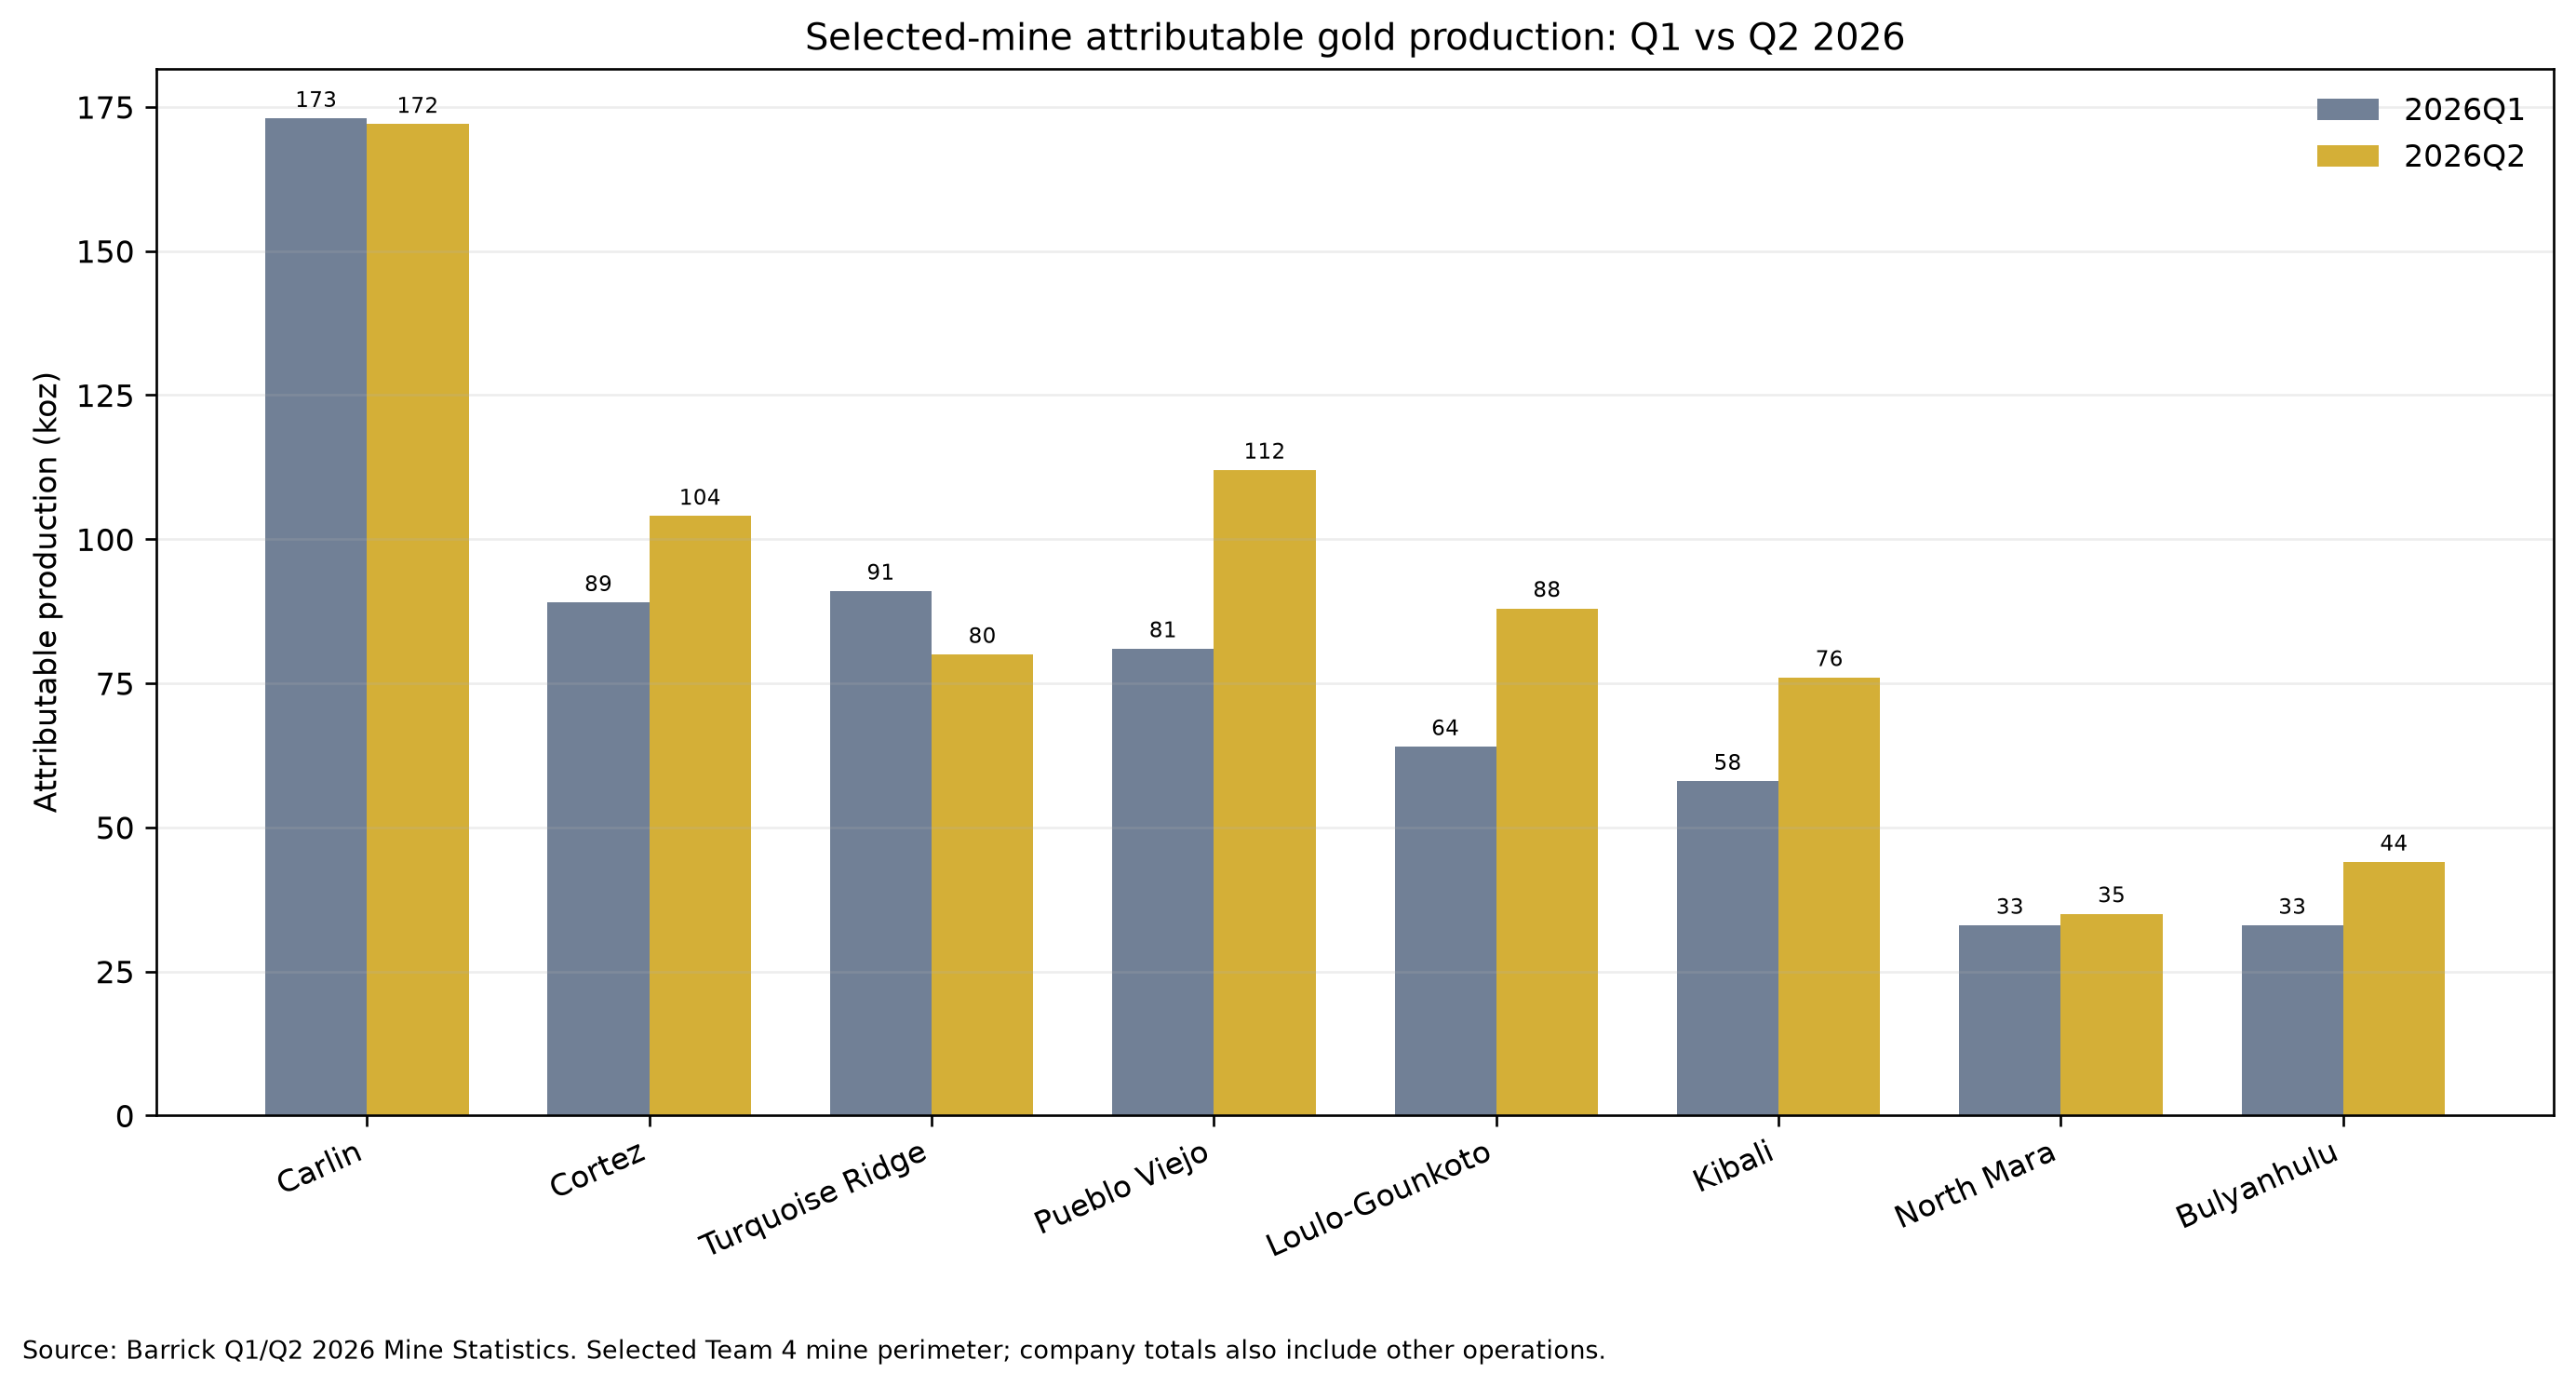
\includegraphics[width=\textwidth]{img/team4_current/team4_mine_production_qoq.png}
    \caption{Attributable gold production for the eight mines retained from
    the Team~4 study, refreshed from Barrick's Q1 and Q2 2026 Mine Statistics.
    These bars are current observations, not simulated production paths.}
    \label{fig:team4-production-qoq}
\end{figure}

\begin{figure}[htbp]
    \centering
    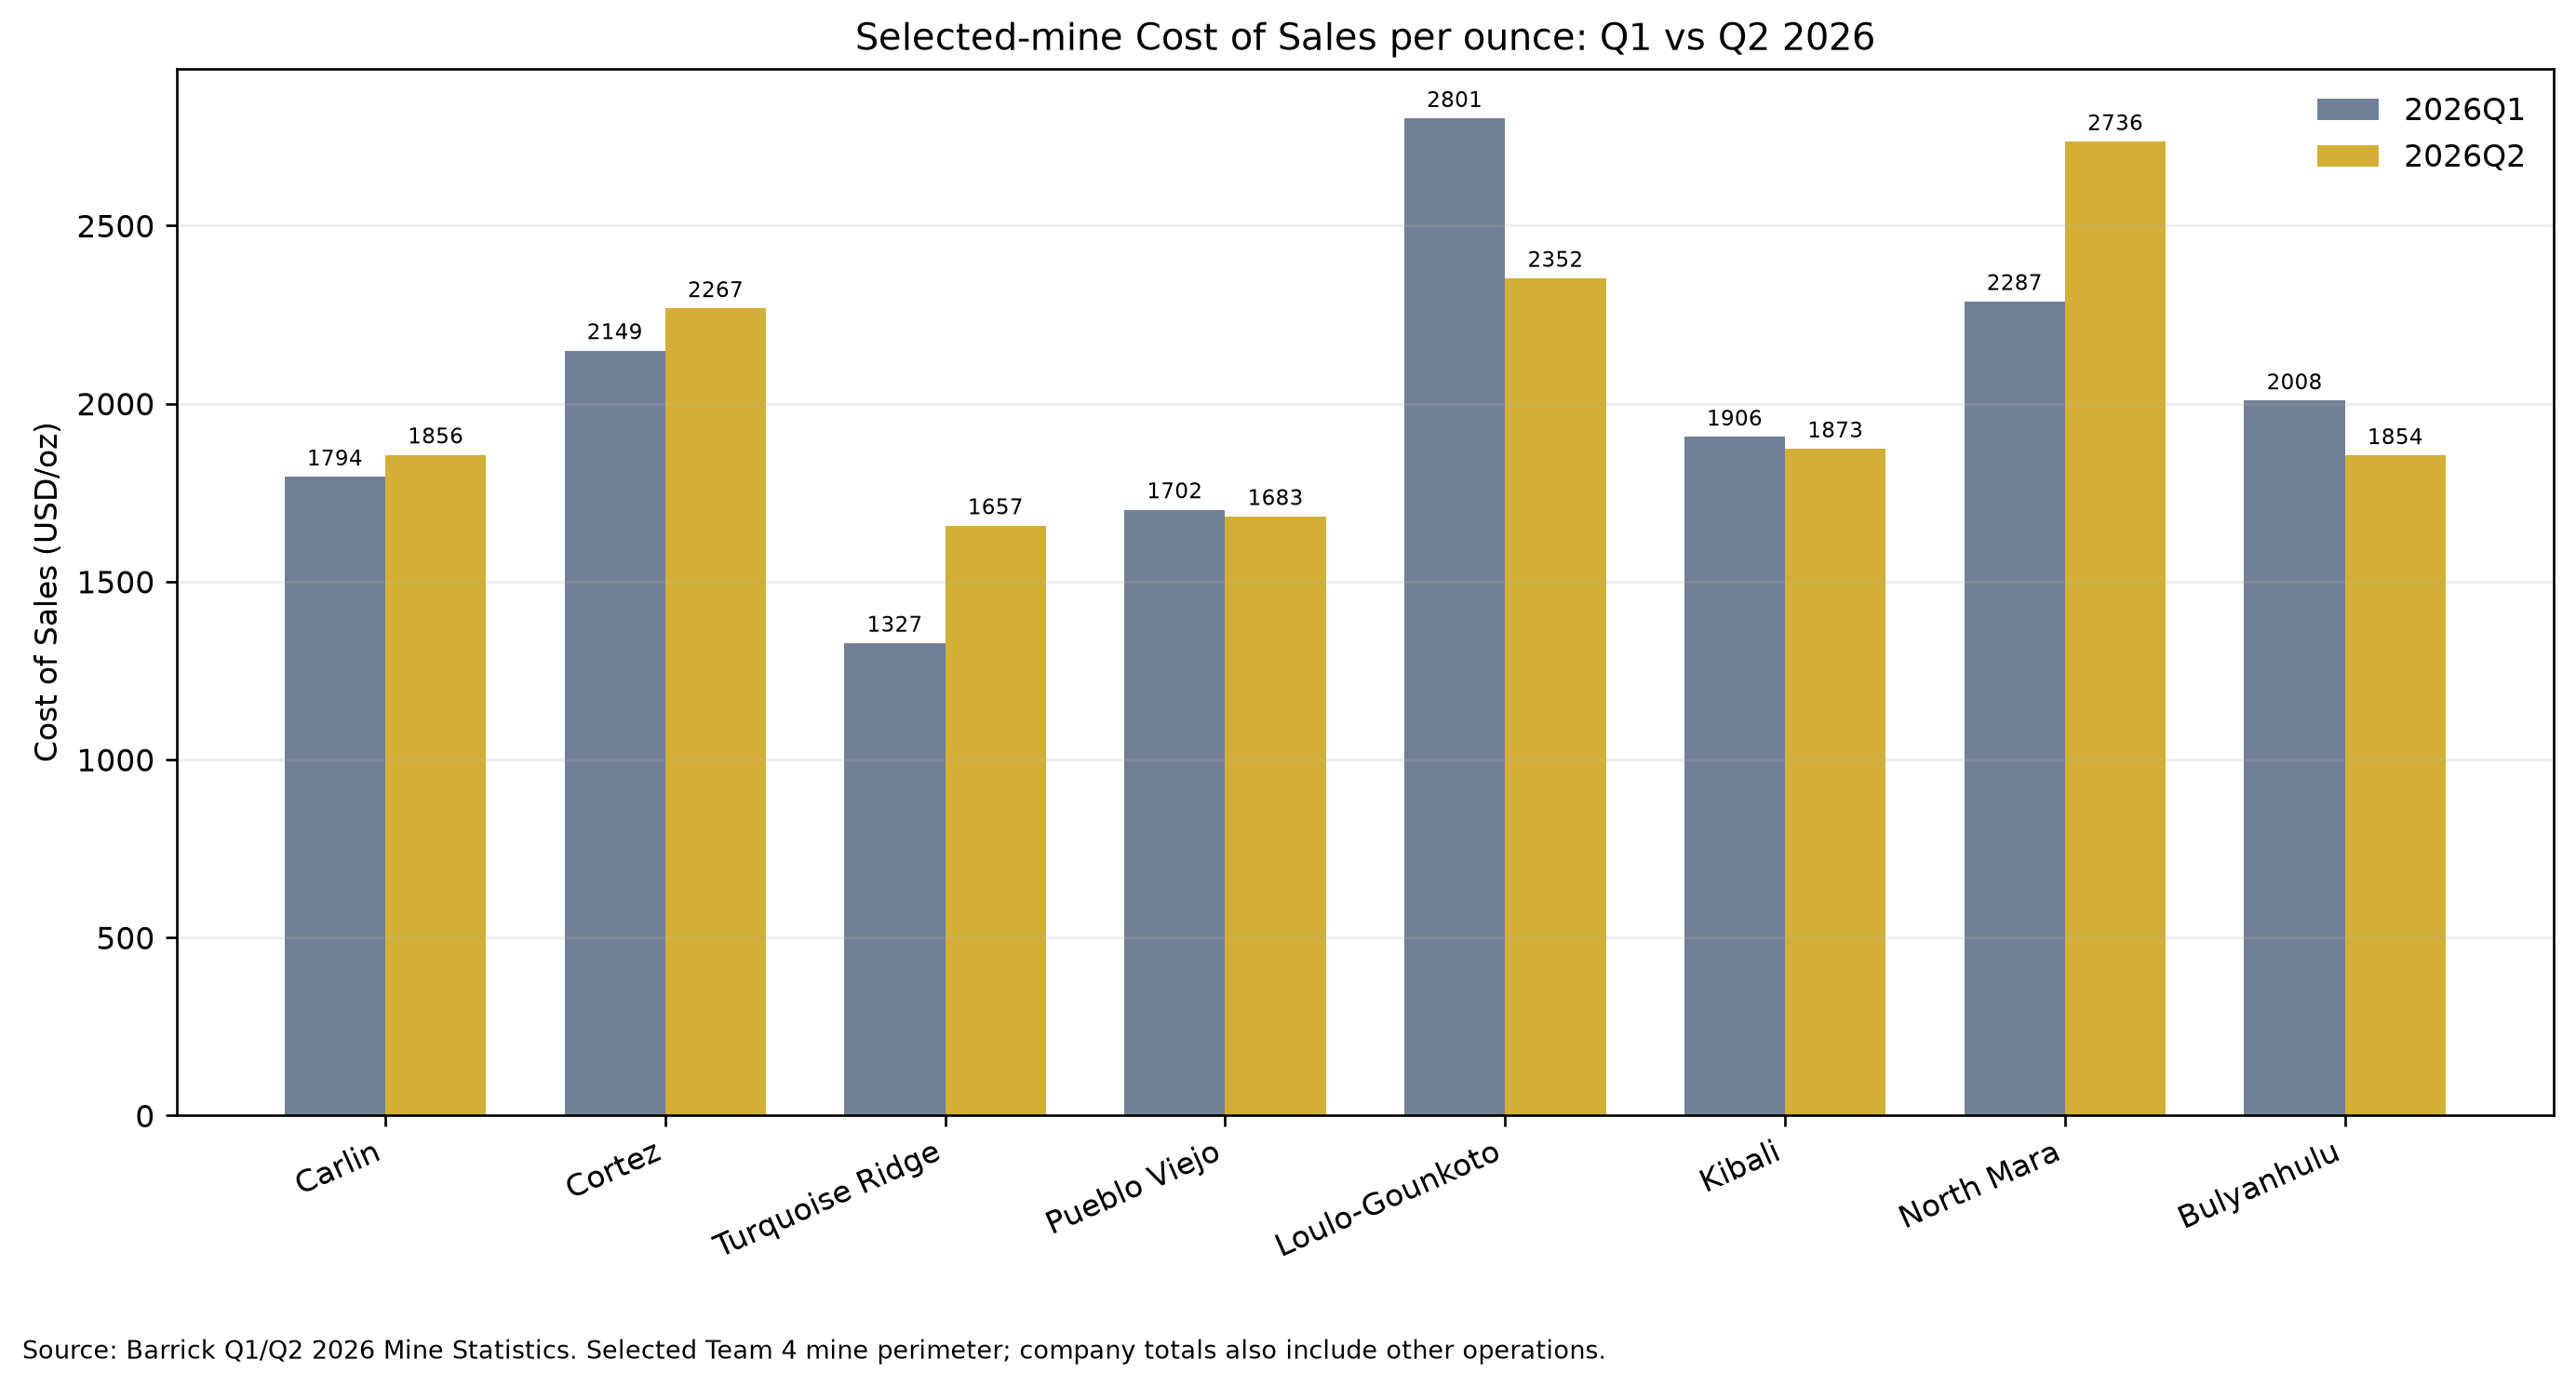
\includegraphics[width=\textwidth]{img/team4_current/team4_mine_cost_qoq.png}
    \caption{Cost of Sales per ounce for the same mine perimeter. The figure
    preserves the Team~4 mine-level comparison while replacing article images
    with a branch-local rendering of current public data.}
    \label{fig:team4-cost-qoq}
\end{figure}

The physical drivers behind production are shown separately in
Figure~\ref{fig:team4-process-components}. This matters because tonnes,
grade and recovery can move in opposite directions: a production change
cannot be interpreted as a price effect, and none of these panels contains a
gold-price input.

\begin{figure}[p]
    \centering
    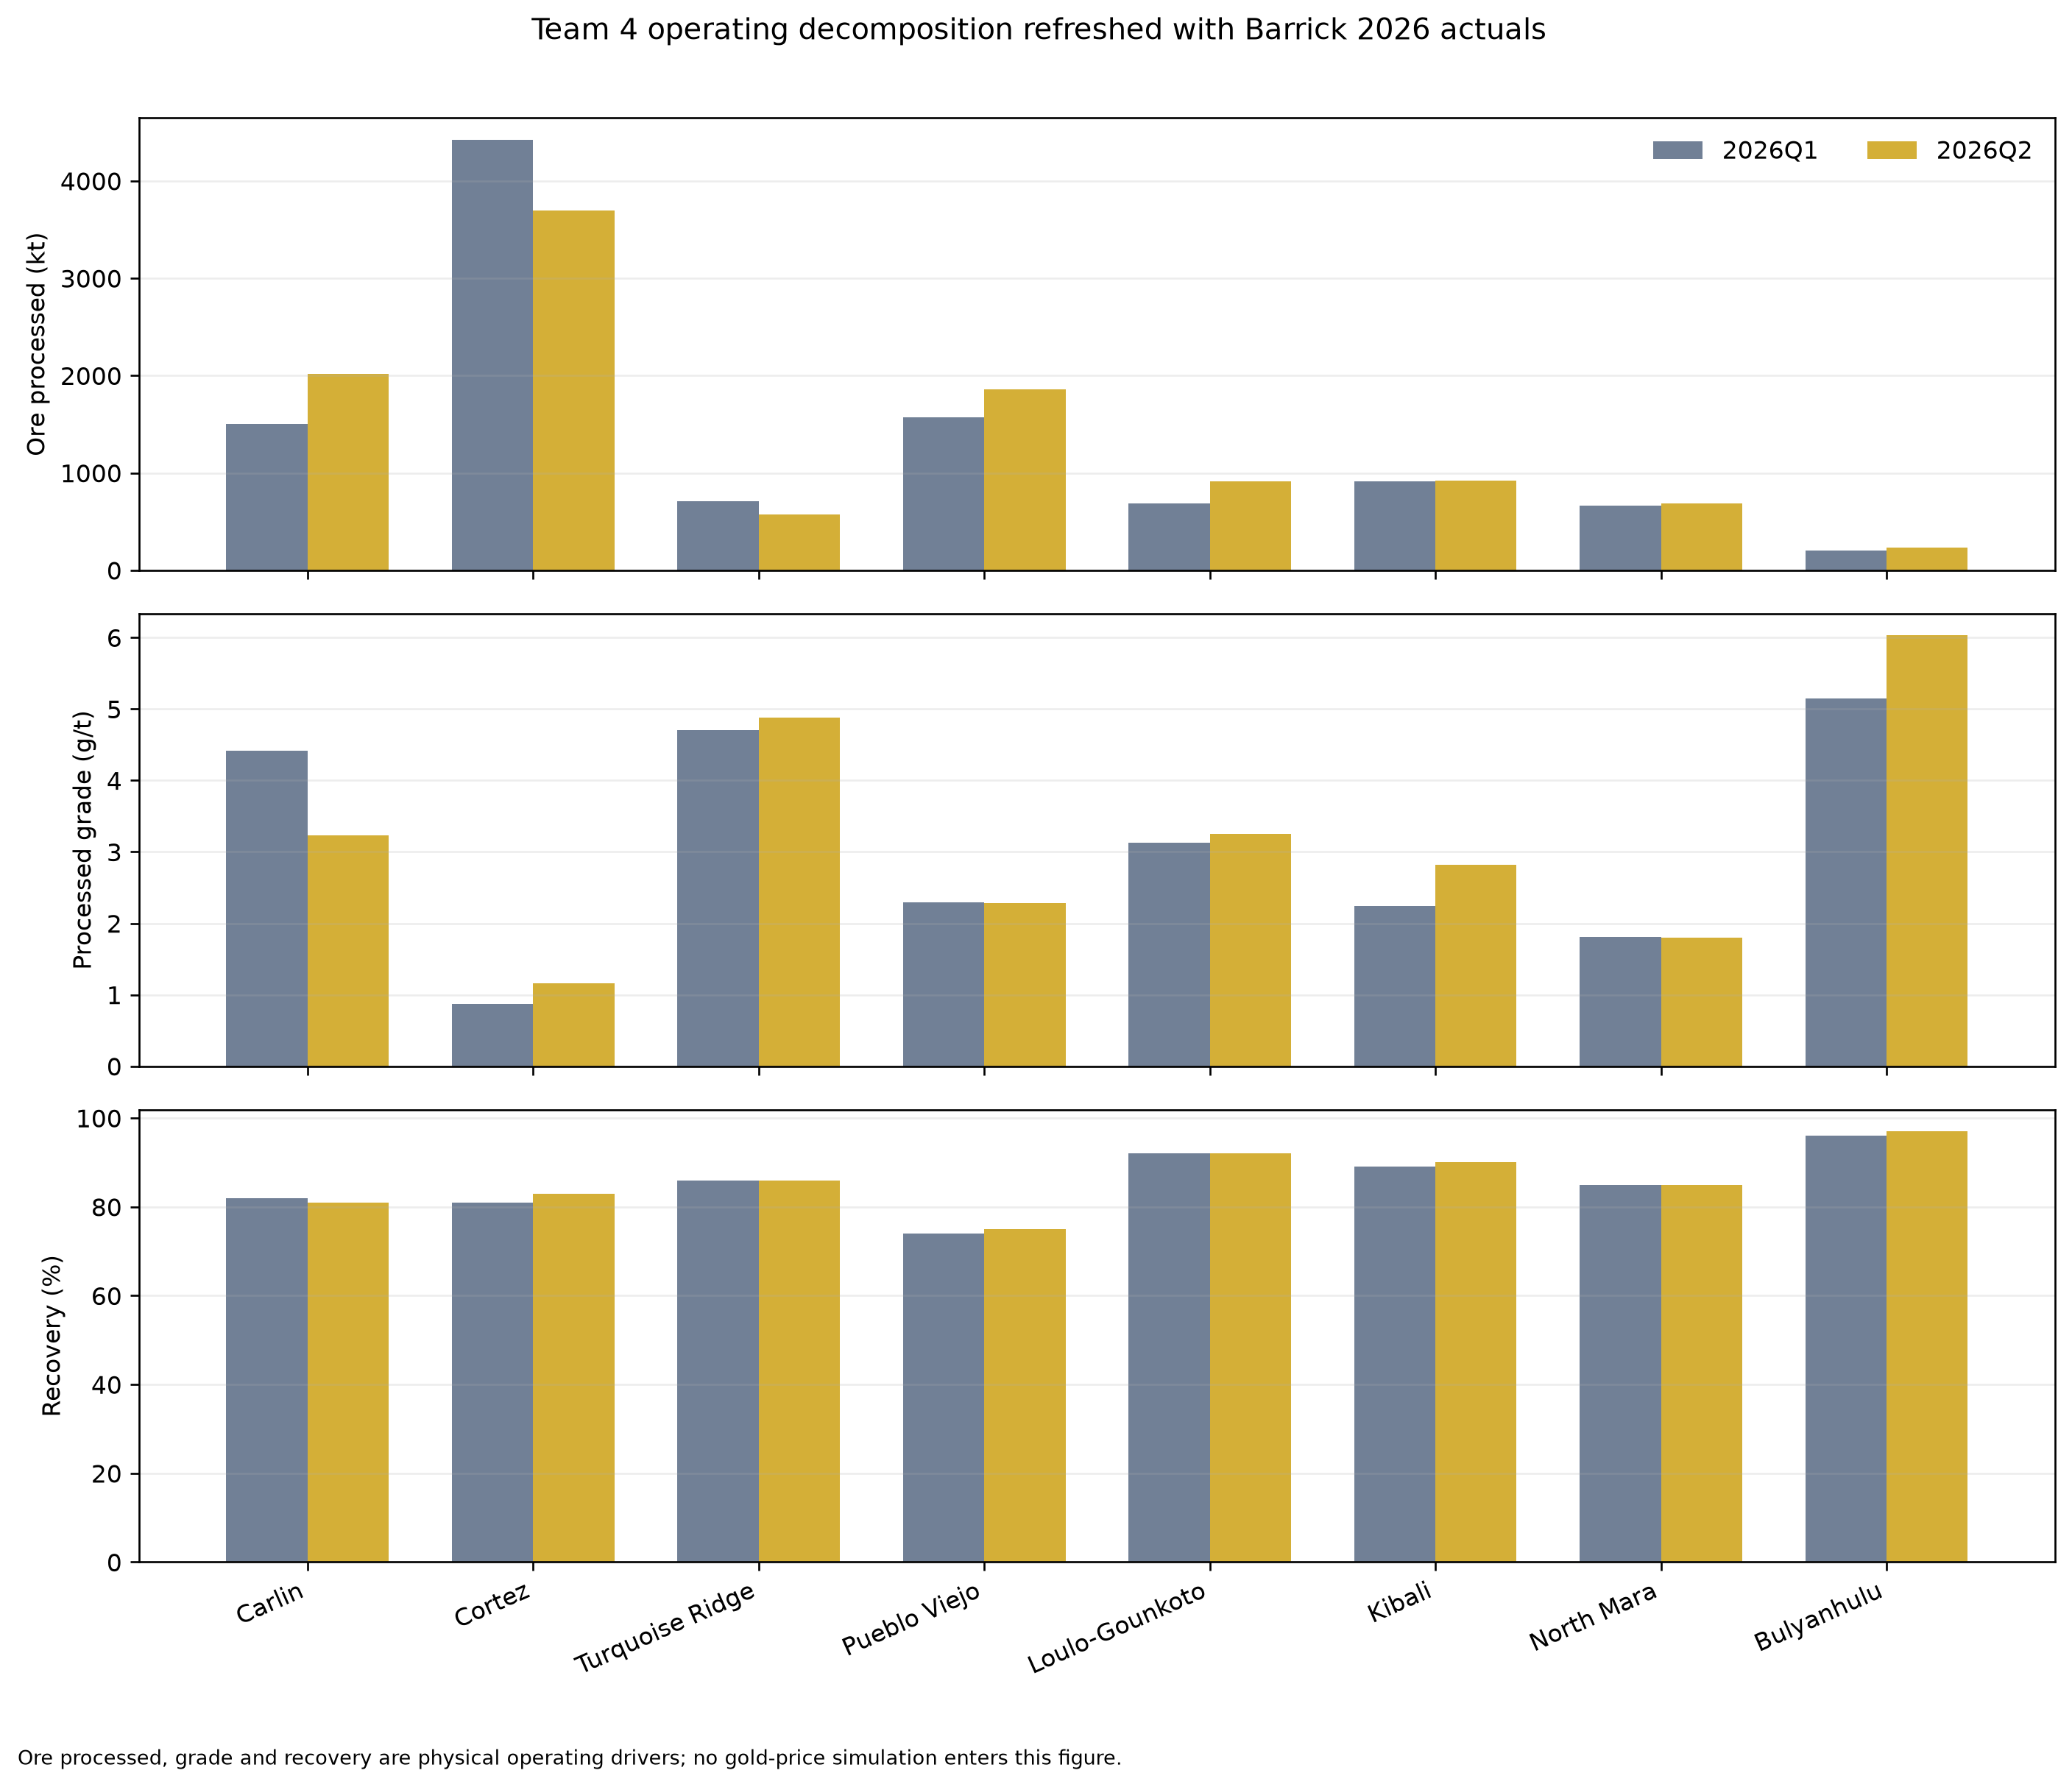
\includegraphics[width=\textwidth]{img/team4_current/team4_process_components_qoq.png}
    \caption{Ore processed, processed grade and recovery in Q1 and Q2 2026.
    Values are transcribed from Barrick's published mine-statistics tables and
    generated by code in this branch.}
    \label{fig:team4-process-components}
\end{figure}

The DCF horizon needs a complete 20-quarter operating vector. The clean
handoff is therefore mixed but explicit: 2026Q1--Q2 are Barrick actuals,
whereas 2026Q3--2030 retain the Team~4 forecasts. Figure~
\ref{fig:team4-operating-contract} marks the boundary in both code and
graphics. This avoids describing a forecast as observed evidence and prevents
the Team~4 price demonstrator from entering the valuation by association.

\begin{figure}[htbp]
    \centering
    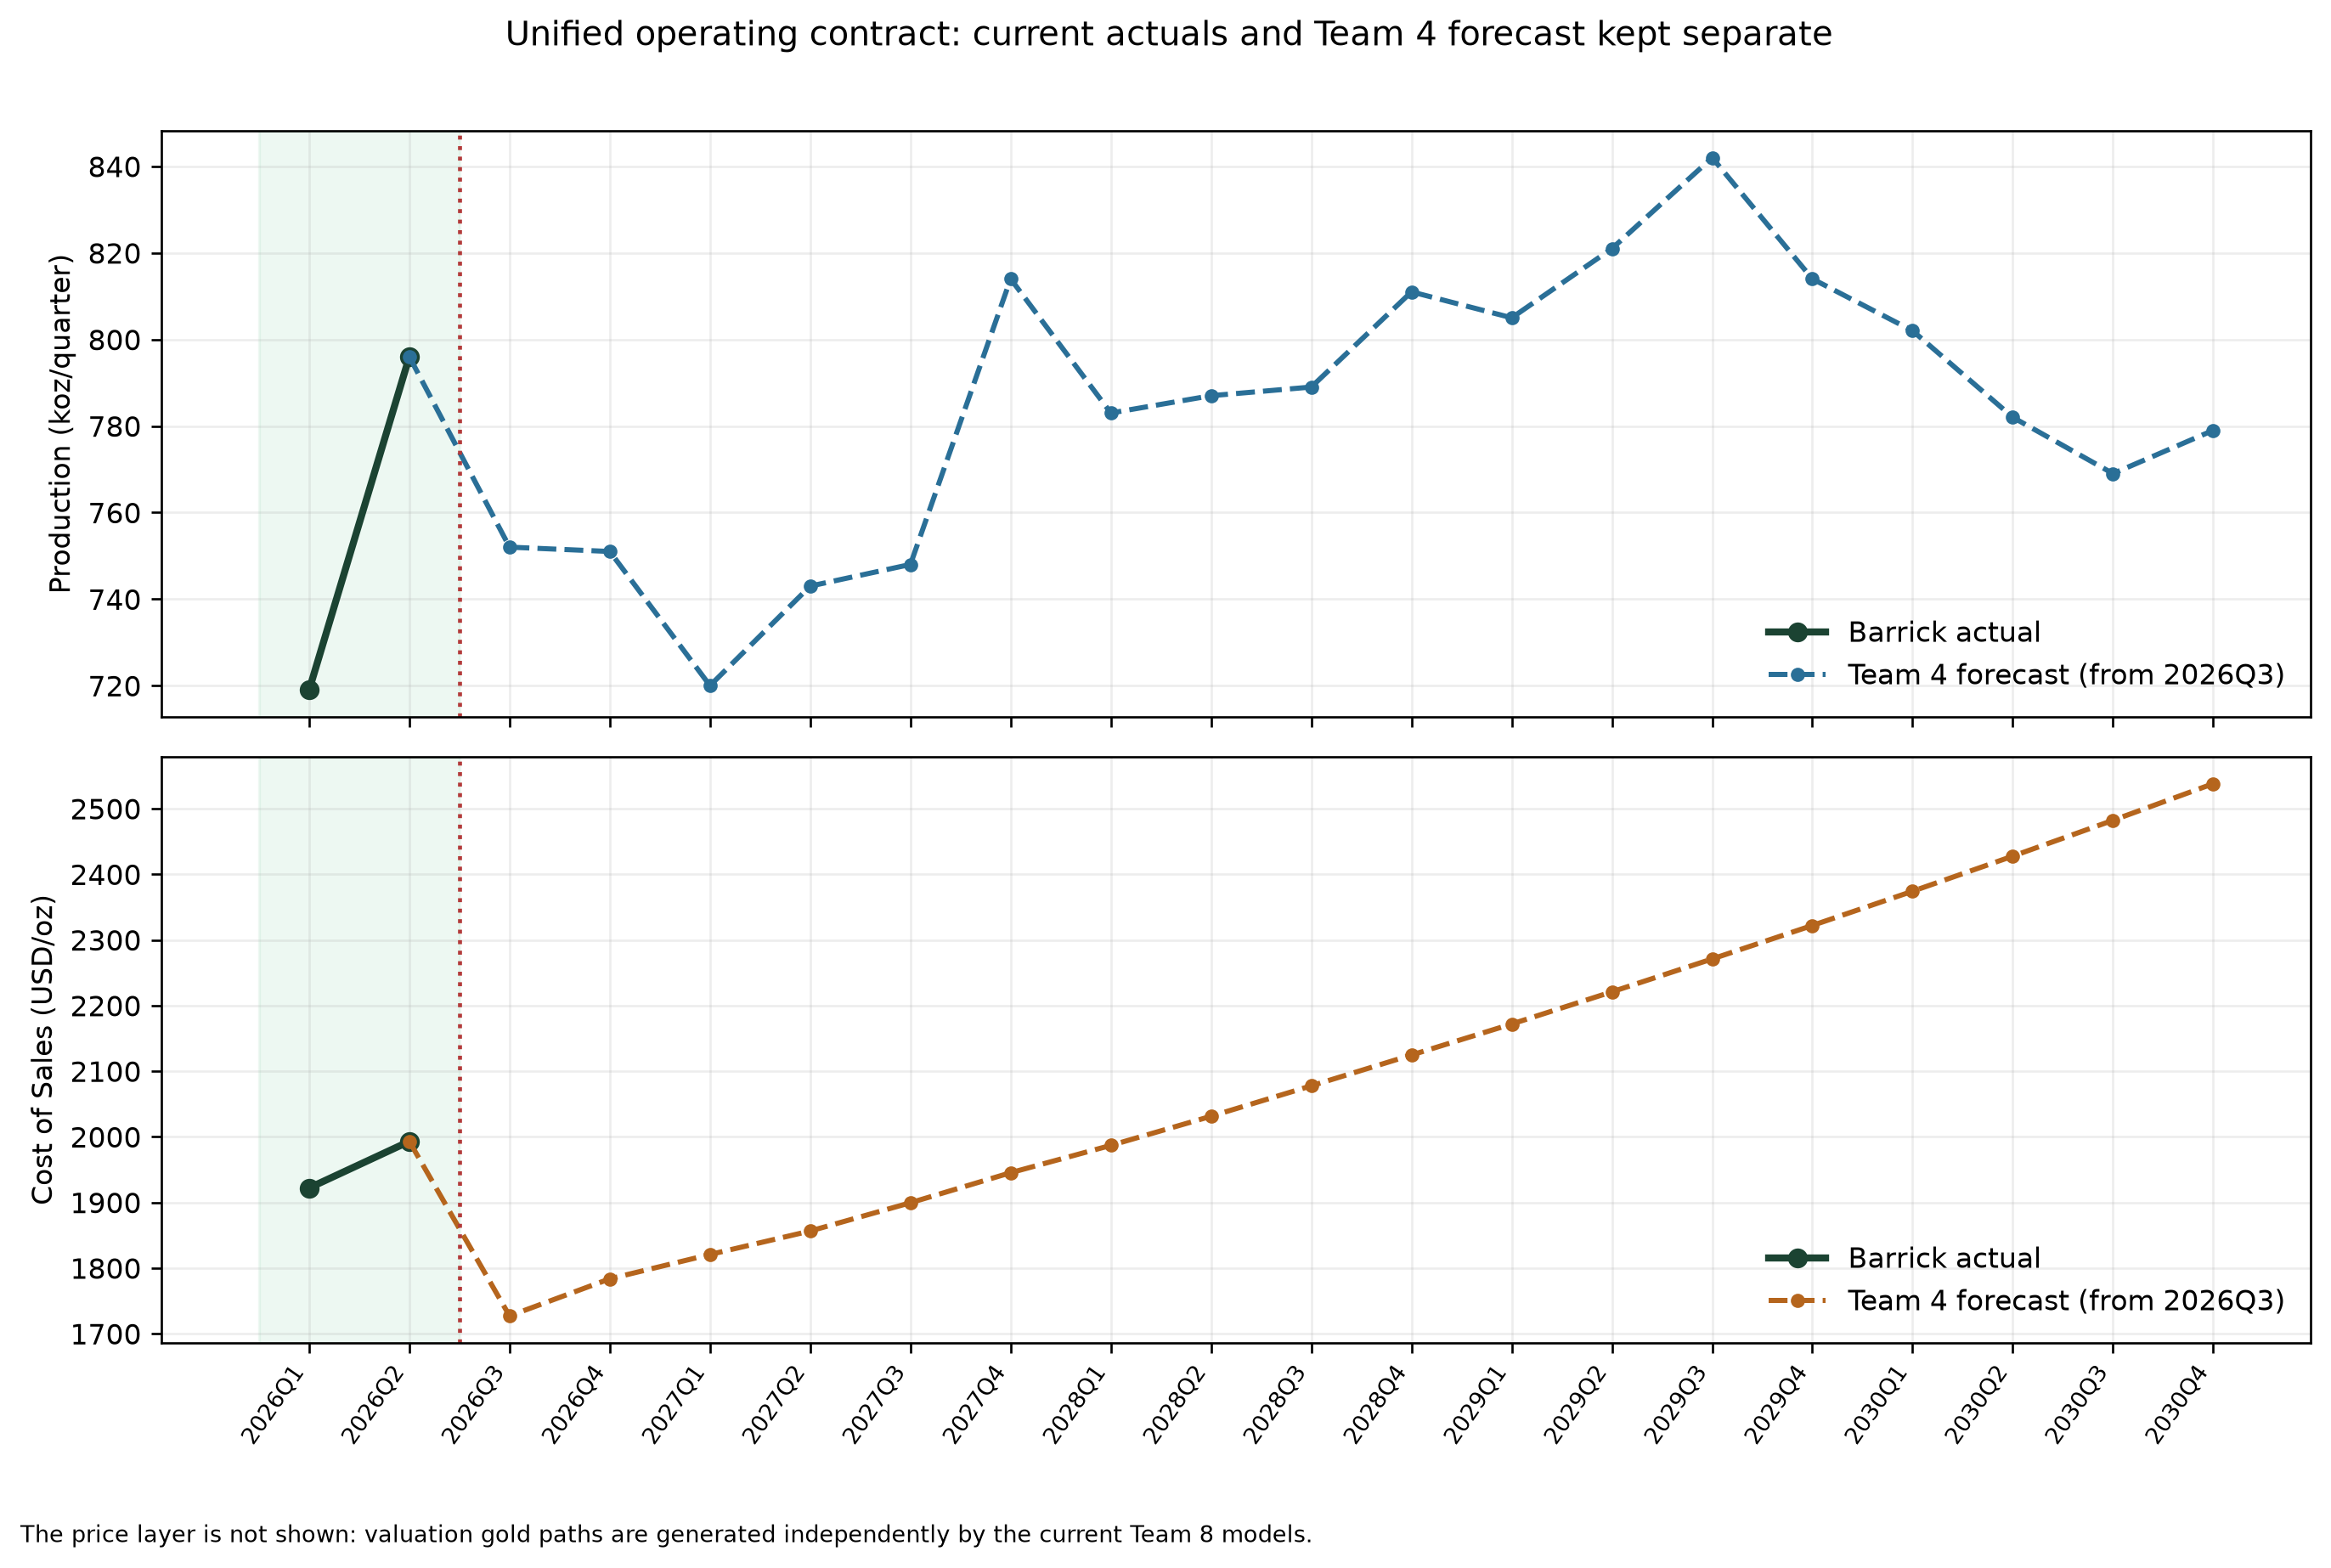
\includegraphics[width=\textwidth]{img/team4_current/team4_operating_contract.png}
    \caption{Operating contract consumed by the unified valuation. Green
    observations are current Barrick actuals; dashed values from 2026Q3 onward
    are Team~4 forecasts. The price layer is absent by design and is supplied
    independently by the current Team~8 models in Chapter~9.}
    \label{fig:team4-operating-contract}
\end{figure}

The remaining operating limitation is economic rather than procedural. The
forecast does not yet model reserves, mine closures, grade-dependent
management actions or endogenous production responses to adverse gold-price
states. Those items remain within the validation boundary and the genuinely
open research agenda; constructing a richer price model is no longer a
Team~4 ``next step'', because that work is already performed in Chapters~8--9.


\section{Handoff to the independent price and valuation layers}

The operating layer ends with production and Cost of Sales. For a quarterly
gold scenario \(P_t\), the pre-reconciliation component margin passed to the
DCF is
\[
    M_t=(P_t-\mathrm{CoS}_t)\,\mathrm{Production}_t .
\]
This identity is retained from Team~4, but \(P_t\) is not generated by the
Team~4 article. Chapter~9 supplies the four current Team~8 price engines and
Chapter~12 performs the corporate valuation. The old NSS--IV--GBM--EBITDA
sequence was useful as a standalone demonstration of an integrated stochastic
DCF; including it here would create a second, incompatible price process and
would blur the provenance of the valuation.

The separation is enforced in three places. First, the branch configuration
uses Barrick's Q2 2026 average realized gold price only as a documented common
level anchor, not as a spot quote or forecast. Second, quarterly risk-neutral
rates come from the current Team~8 LSE Treasury input rather than the Team~4
NSS fit. Third, all simulated paths come from Black--Scholes, Heston,
Bates--Poisson or Bates--Hawkes under one common conditional bridge. Thus
Team~4 contributes operational mechanics and forecasts only; it contributes
no simulated gold price and no standalone valuation output.

\subsection{Limitations carried forward}

The 2026Q1--Q2 refresh removes the earlier lack of current operating evidence,
but it does not turn the later Team~4 values into management guidance. From
2026Q3 onward they remain research forecasts. Mine depletion, reserve lives,
closures, recovery interventions, cost inflation by jurisdiction and
price-dependent management actions are not endogenous. These are live model
limitations. By contrast, richer stochastic volatility and jump models are
not future work for this chapter: they have already been implemented and
tested in Chapters~8--9, then propagated through the unified experiment in
Chapter~12.
